\subsection{UPnP}
\label{subsec:upnp}
O \emph{Universal Plug and Play Protocol} (UPnP) é um protocolo para conectividade entre aplicações inteligentes utilizado em computadores e dispositivos, \emph{wireless} em geral. Foi definido com o objetivo de facilitar a conectividade entre dispositivos em diferentes ambientes, como casas, pequenas empresas ou espaços públicos~\cite{upnpArch}. Não necessita de configurações e fornece uma rede invisível com descoberta automática de dispositivos de diferentes fabricantes e diversas categorias.

Seu nome ``Universal'' advém da não utilização de \emph{drivers} para cada dispositivo. Para tal, utiliza protocolos bem conhecidos como IP, TCP, UDP e HTTP, além do formato XML, utilizado no armazenamento de informações tais como fabricante, lista de dispositivos embarcados, descrição dos serviços com lista de comandos e ações com parâmetros e argumentos, URL's de controle, eventos e apresentação.

Quando um novo aparelho adentra na rede, ele recebe um IP via DHCP ou gera um IP para si (no caso de redes não-gerenciadas), publica seus serviços, disponibiliza uma URL e conhece os serviços de outros dispositivos. A \emph{UPnP Device Architecture}(UDA) divide os dispositivos em duas categorias principais: controlados, também chamados de ``dispositivos'' e pontos de controle~\cite{upnpArch}, estabelecendo uma arquitetura cliente-servidor onde pontos de controle acessam os serviços disponibilizados pelos dispositivos. Após a entrada desse novo aparelho na rede, os pontos de controle ainda não têm muita informação sobre o dispositivo, então os pontos de controle interessados solicitam a descrição do dispositivo por meio da URL disponibilizada anteriormente.

O UPnP estabelece uma classificação utilizando um conjunto de tipos pré-determinados. Quando um fabricante deseja produzir um novo dispositivo, este deve se adequar a estes tipos ou estabelecer um novo tipo próprio. Uma característica interessante dessas classificações é que elas podem ser implementadas por dispositivos com pouca capacidade de computação, embora também possam ser utilizadas por dispositivos mais robustos como computadores, ou seja, são independentes de plataforma. Os tipos presentes no UPnP são:

\begin{itemize}
\item Áudio/Vídeo:

	Essa categoria possui duas principais sub-classificações que foram sendo atualizadas com o surgimento de novas tecnologias: 
	\begin{itemize}
		\item \emph{Media Server}:

			Define um dispositivo genérico que provê conteúdo de áudio e/ou vídeo, como CD e DVD \emph{players}, cameras, rádios, televisões e \emph{set-top boxes}. Embora, seja utilizado por dispositivos com diferentes capacidades de processamento, diferentes conteúdos e em diferentes formatos, o \emph{Media Server} expõe o conteúdo disponível de forma uniforme e consistente por meio de um Diretório de Conteúdo.

		\item \emph{Media Renderer}:

			Define um dispositivo genérico capaz de renderizar conteúdos de áudio e/ou vídeo como MP3 \emph{players} e televisões. Dependendo da implementação de um \emph{Media Renderer}, pode-se utilizar os recursos de auto-falante de uma televisão para consumir um serviço de música de um \emph{Media Server}.
	\end{itemize}
\item Gerenciamento de Dispositivos:

	Essa categoria foi criada para adicionar operações gerenciais à qualquer dispositivo UPnP. Essa gerência inclui funções para configuração de serviços e do próprio dispositivo, diagnóstico e correção de problemas além de gerência do \emph{firmware} e dos \emph{softwares} do dispositivo.

\item Automação Residencial:

	O UPnP define quatro tipos de dispositivos de automação residencial:
	\begin{itemize}
		\item Cortina de Proteção Solar:

			Provê uma sombra por meio de uma cortina. Seu controle pode ser manual, automático ou desabilitado. Sua especificação não contempla configurações a respeito da automação da cortina ou proteções.
		\item Câmera Digital de Segurança:

			Provê controle básico sobre a configuração da câmera, contendo serviços de fotos e vídeos.
		\item Aquecimento, Ventilação e Ar-Condicionado:
			
			Esse dispositivo conta com auxílio de sensores de temperatura e possui a capacidade de saber ou controlar a temperatura do ambiente por meio de ventiladores e ar-condicionados.
		\item Controles de Luz:
			
			São divididos em \emph{Luz binária}, que representa uma lâmpada ou qualquer dispositivo emissor de luz que possa somente estar apagado ou aceso, e em \emph{Luz} cuja intensidade pode ser alterada, 
	\end{itemize}

\item Rede:

	Nessa categoria se enquadram dispositivos relacionados com uma rede, seja um \emph{gateway} ou um ponto de acesso local.
	\begin{itemize}
		\item \emph{Gateway} de Internet:
			
			Essa classificação define um dispositivo de interconexão entre uma \emph{Local Area Network} (LAN) e a \emph{Wide Area Network} (WAN), provendo conectividade com a internet.
			\begin{itemize}
				\item Dispositivo de Conexão WAN: É um dispositivo virtual definido tendo o \emph{Gateway} de Internet como raiz. Funciona como um contêiner para um \emph{link} ou serviços de conexão em uma interface WAN. 
				\item Dispositivo WAN: É um dispositivo virtual definido tendo o \emph{gateway} de internet como raiz. Cada dispositivo WAN é uma instância virtual de uma interface WAN no \emph{gateway} de internet. Múltiplas interfaces físicas WAN para clientes UPnP, existirão distintas instâncias deste dispositivo.
			\end{itemize}

		\item Ponto de acesso WLAN(\emph{Wireless Local Area Network}):
			
			Esse dispositivo implementa os padrões IEEE 802.11 (a,b,g) sem fio para prover uma infraestrutura de rede para casas e pequenas empresas. Essa definição não inclui uso dos pontos de acesso como \emph{hotspots} ou redes de grandes empreendimentos. O ponto de acesso age como uma ponte \emph{Ethernet} que permite ligações de múltiplos nós com a LAN.
	\end{itemize}

\item Impressora:

	Define um dispositivo com capacidade de impressão. Essa especificação não abrange dispositivos que possuem funções de FAX ou \emph{Scanner}, que possui uma especificação própria.

\item Acesso Remoto:

	Essa categoria comporta dispositivos que gerenciam o acesso remoto, ela é dividida entre:
	\begin{itemize}
		\item Agente de Descoberta de Acesso Remoto:

			Possui a função de prover a capacidade de sincronizar a informação sobre a descoberta UPnP entre duas redes remotas.
		
		\item Servidor de Acesso Remoto:
		
			Permite que pontos de controle configurem Servidores de Acesso Remoto.

	\end{itemize}

\item Interface Remota:

	Classifica dispositivos entre servidores e clientes de uma interface remota com o usuário.

\item \emph{Scanner}:

	Representa um dispositivo de \emph{Scanner} com \emph{feeder} opcional. Esse dispositivo possui os serviços de digitalização via \emph{feeder} ou \emph{flatbed} e um serviço para configuração com o painel frontal do dispositivo. Essa categoria não contempla funcionalidades de Fax ou cópias.

\item Telefonia:
	
	Categoria para aparelhos que se relacionam com algum serviço de telefonia, tanto como consumidor quanto como con provedor.
	\begin{itemize}
		\item Servidor de Telefonia:

			Permite que pontos de controle gerenciem chamadas telefônicas, mensagens e presença por meio de outros dispositivos UPnP. 

		\item Cliente de Telefonia:
		
			Permite que pontos de controle possam gerenciar mídias por meio de um de um servidor de telefonia.
				
	\end{itemize}

\item Básico:

	A definição de dispositivos básicos provêem um mecanismo para produtos que não se enquadram em uma classificação adequada do UPnP, possam utilizá-lo. Por esse motivo, essa especificação não possui nenhum serviço definido, mas pode ser utilizada como dispositivo raiz para outras categorias já definidas.
\end{itemize}

\begin{figure}[ht]
\center
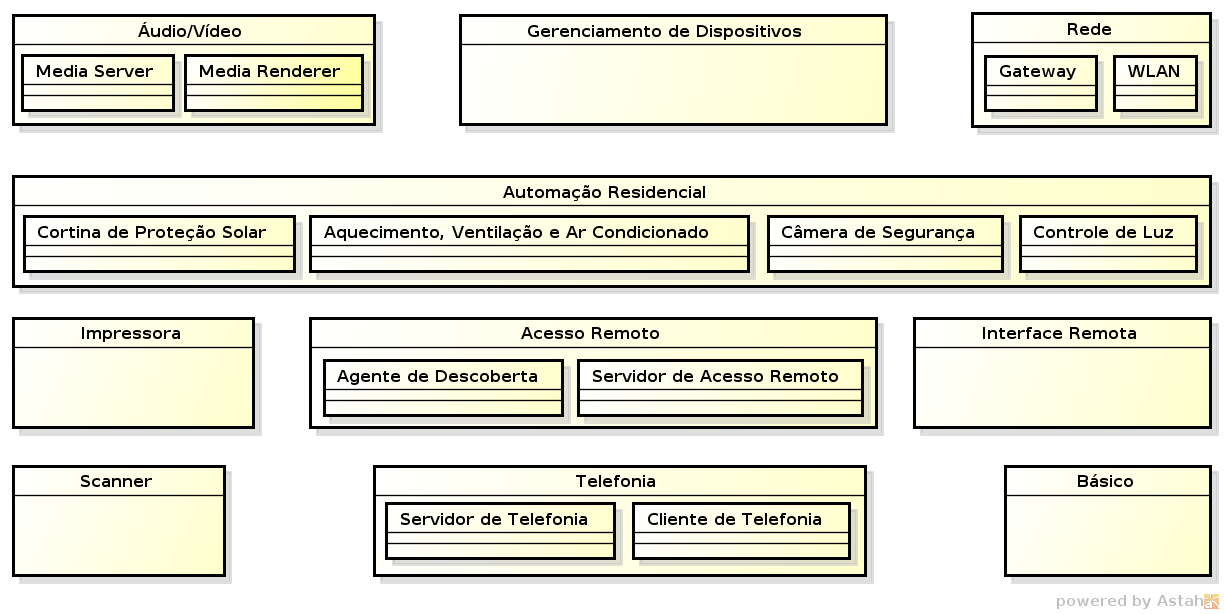
\includegraphics[scale=0.49]{imagens/recursosUPnP}
\caption{Representação gráfica dos tipos existentes no UPnP.}
\label{fig:ddlspec}
\end{figure}

A partir de uma classificação padrão, os fabricantes podem, por exemplo, estender e especializar determinada definição adicionando novos serviços, o que sugere a formação de uma hierarquia de dispositivos por meio de arquivos XML. O UPnP, portanto, utiliza uma classificação de dispositivos relacionada, o que facilita a criação de novos tipos de dispositivos a partir da classificação base agregando novos serviços. Essa classificação extendida, entretanto, deve passar por um processo de certificação. Um ponto forte nas classificações é o fato de já incluirem a especificação dos serviços que os dispositivos provêem.

De volta ao exemplo apresentado no início deste capítulo, observa-se que as televisões citadas classificariam-se como dispositivos de áudio e vídeo.